\setchapterpreamble[u]{\margintoc}
\chapter{Why Quantum Mechanics?}
\labch{intro}

Born out of the failure of classical physics to explain everyday phenomenon, quantum mechanics, and its extension to quantum field theory, is one of the most powerful and predictive theories in physics to this day. Understanding quantum mechanics has led to technological developments that range from laser barcode scanners to MRI machines. The promises of quantum mechanics in the future include new paradigms of computing and sensing. The goal of this introductory chapter is to gain an appreciation for the key conceptual ideas of quantum mechanics and its applicability in the everyday world.

\section{Waves as Particles: The photoelectric effect}

In a classical wave (think of water or the string of a violin), the energy of the wave is related to its amplitude. A higher wave carries more energy, and if a violin is plucked harder, it'll sound louder. This holds true, even for electromagnetic waves which have energy density given by

\begin{equation}
\mathcal{E}_{\text{EM}} = \frac{1}{2}\epsilon_0 |\mathbf{E}|^2 + \frac{1}{2\mu_0} |\mathbf{B}|^2 
\end{equation}

However, experiments performed in the late 19th century began to change this perception. In 1887, Hertz discovered that ultraviolet light, whose distinguishing feature is its high \textit{frequency} not amplitude, could create vigorous sparks between metal electrodes. The ejection of electrons from a material due to light was dubbed the \textbf{photoelectric effect}, and was a beautiful confirmation of the relationship between light and electromagnetism, a cornerstone of Maxwell's theory. 

In 1902, Lenard set up an ingenious experiment to measure both the \textbf{number} and \textbf{energy} of the ejected electrons from a metal due to a source of light. The ejected electrons from the metal were guided to a collector and the current was measured with a precision ammeter. The energy of the electrons was measured by applying a potential $V_{\text{stop}}$ to the collector to repel the electrons. What Lenard found was that by increasing the brightness (amplitude) of the light source, the current increased, but $V_{\text{stop}}$ was unaffected! In fact, the frequency of light impacted $V_{\text{stop}} $, where higher frequencies required larger stopping potentials. This confirmed Hertz's earlier observation of the potency of ultraviolet light. 

\begin{marginfigure}[-12cm]
	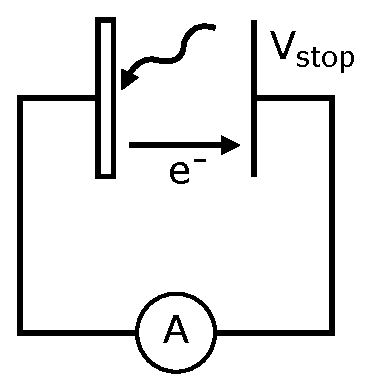
\includegraphics{images/chap1_photoelectric.eps}
	\caption{A schematic of Lenard's experiment. Light ejects electrons off of a metal towards an electrode. After hitting the electrode, a current is readable on the ammeter. A stopping potential $V_{\text{stop}} $ can be applied to measure the energy of the ejected electrons.} 
	\labfig{photoelectric}
\end{marginfigure}

These observations were finally explained by Einstein in 1905\sidenote[][-12mm]{This year was known as Einstein's \textit{annus mirabilis} (or miracle year). Einstein published 4 papers: an explanation of the photoelectric effect, Brownian motion, special relativity, and the mass-energy equivalence. He won the Nobel Prize in 1921 for the photoelectric effect. Let us all have our miracle years!}. He postulated that the energy from light must come from \textit{packets} or \textit{quanta}. Each quantum of light has energy that is proportional to frequency 

\begin{equation}
E = h\nu 	
\end{equation}

where $ h $ is the Planck constant\sidenote{Max Planck introduced this constant to explain the blackbody radiation spectrum and solve the ultraviolet catastrophe in 1900. This experiment is another key result in the beginnings of quantum mechanics.}. Ultraviolet light, which is at a higher frequency, imparted more energy on each ejected electron, while the amplitude increased the \textit{number} of quanta, and hence the number of elected electrons (the current in Lenard's experiments). It is worth noting here that an increased amplitude \textit{does} increase the energy (there is no conflict with classical thinking), but it increases it via the \textit{number} of quanta. Each quanta's energy is related to its frequency.

With the introduction of energy quanta, it became clear that light, which was classically thought of as a wave, \textit{also has particle like behavior}. These particles of light became known as \textbf{photons}. Each photon also has a momentum given by 

\begin{equation}
	p = \frac{E}{c} = \frac{h\nu}{c} = \frac{h}{\lambda} \label{eq:photon-momentum}
\end{equation}

where $ E = pc $ is the energy of a massless relativistic particle, $c$ is the speed of light and $\lambda$ is the wavelength.

\section{Particles as Waves: Interference of individual electrons}

Now, we discuss a situation where particles can exhibit wave-like behavior, which is at the heart of the description of quantum mechanics. Another classical wave phenomenon is interference. Wave amplitudes can add together constructively to create larger waves, but also cancel each other destructively. Applying this principle to waves sent through multiple slits give rise to interference patterns. Thomas Young, in 1803, demonstrated that light was a wave by experimentally verifying these interference patterns.
\begin{marginfigure}[-7cm]
	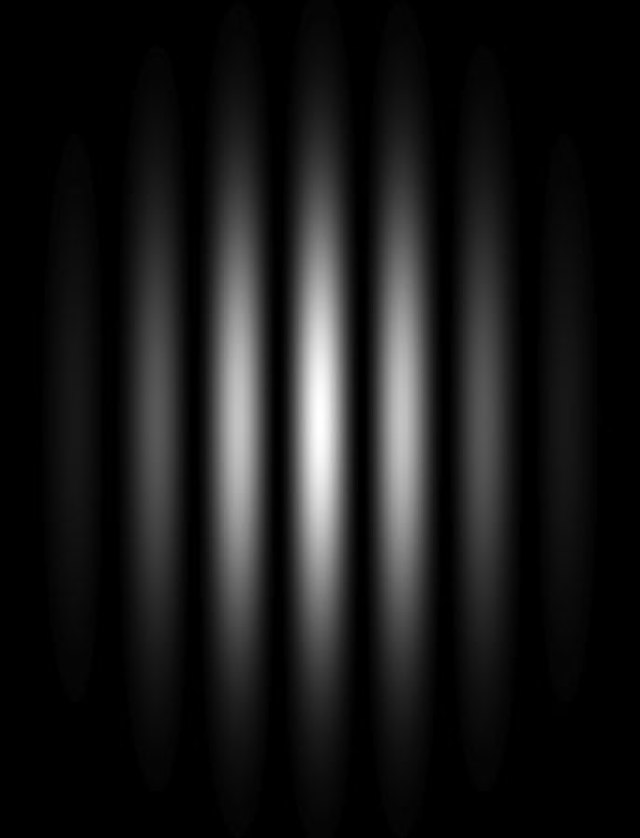
\includegraphics{images/double_slit_simulated.jpg}
	\caption{A simulated image of the interference pattern when light passes through two slits. Bright stripes correspond to locations of constructive interference, and dark stripes correspond to locations of destructive interference. Without interference, only two spots are expected at the location of the two slits. } 
	\labfig{double_slit}
\end{marginfigure}

However, would particles, such as electrons, exhibit such behavior? In 1927, Clinton Davisson and Lester Germer showed that when electrons are diffracted off a crystal of Nickel, an interference pattern due to its crystal structure was visible in the locations of the diffracted electrons. A double-slit experiment was finally performed by Claus Jonsson in 1961 further confirming that electron beams did exhibit wave-like behavior. Perhaps most surprisingly, Pier Giorgio Merli, Giulio Pozzi and GianFranco Missiroli in 1976 performed a double-slit experiment with \textit{single} electrons. Although one might conceive that beams of electrons can contain individual electrons which interfere with others, Merli, Pozzi and Missiroli's experiment showed that single electrons also \textit{interfere}, and they interfere with themselves\sidenote{Akira Tonomura and colleagues at Hitachi performed a single-electron double-slit experiment in 1989. A video is available on YouTube, where you can see the electrons accumulating one at a time, yet together they eventually display an interference pattern. I encourage you to look it up!}! In fact, this is in agreement with quantum mechanics where individual particles are treated as having \textbf{wavefunctions} and being waves themselves. 

Just as light can have a momentum which is related to its wavelength, massive particles have a wavelength that is associated with its momentum. Letting $ p = mv $ and using equation \ref{eq:photon-momentum}, we can solve for the \textbf{de Broglie wavelength}

\begin{equation}
	\lambda = \frac{h}{mv}
\end{equation}

For massive particles, like electrons, to diffract, the size of the slits must be on the same order as the de Broglie wavelength. The idea that particles can behave like waves and waves can behave like particles is known as \textbf{wave-particle duality}\sidenote[][-6mm]{As we will see in this book, quantum mechanics places an emphasis on treating particles like waves. In this sense, particles have a very special place, as wavefunctions are written for particles or collections of particles. However, in many high energy processes, particles can be created or destroyed. The key insight in \textbf{quantum field theory} is that the fundamental objects are actually quantum fields that pervade all space. Particles are merely excitations in the quantum field. This is a topic for another course.}. This surprising experimentally based discovery required a new understanding of physics and led to the theory of quantum mechanics. 

As we begin to think of particles like waves and waves like particles, it is important to stop briefly for a philosophical interlude. It is easy to get caught up in what is truly physical reality or what is actually happening, which is often rooted in one's daily experiences. Unfortunately, daily experiences are heavily influenced by the laws of classical mechanics, which is precisely why theories like electromagnetism and quantum mechanics\sidenote{For more information, I recommend Peter Dear's book, The Inteligibility of Nature.} were difficult to accept and required paradigm shifts. To avoid these hairy issues, I advise you to always remember that quantum mechanics is indeed \textit{backed up by real physical experiments}. Regardless of the exact interpretations (which might be held back by classical conceptions), our goal is to develop a predictive and explanatory framework for physical phenomenon. This goal is not impeded, no matter how one might want to interpret the results, as long as the same results are acquired. With that prelude, we now turn to gain more intuition on how quantum phenomenon \textit{are} actually present in everyday phenomenon, and can start forming the basis for some intuition.  

\section{Line Spectra in Atoms}

Another one of the first areas in nature where features of quantum mechanics were elucidated was in the spectra of atoms. The concept of an atom, from the Greek \textit{atomon}, meaning indivisible, was first introduced by Democritus in ancient Greece. He proposed that atoms made up all matter, and this theory gained steam in the 19th century, where a collection of scientists including Antoine Lavoisier verified the composition of water being two parts hydrogen and one part oxygen. Through explorations of cathode rays, J.J. Thompson in 1897 concluded that atoms were divisible after all and included subatomic particles, like negatively charged electrons. The discovery of the electron was awarded the Nobel Prize in 1906. Attention then turned to the structure of the atom. These electrons were initially thought to be evenly distributed across a positively charged background that composed the atom, and was coined the \textit{plum pudding model}. In 1911, Ernest Rutherford bombarded gold foil with alpha particles, and found that most particles passed straight through. This experiment confirmed that the atom was mostly empty space, and he posited that a positively charged nucleus was concentrated in the center of the atom. Around the same time and earlier, scientists discovered that light is composed of different colors, and that gases of certain chemical elements emitted light of particular colors or frequencies. Using the insight from Einstein, these frequencies correspond to a discrete set of energies. In order for atoms to emit only a discrete spectrum, Niels Bohr postulated that electrons orbited the nucleus at fixed distances, which corresponded to a discrete set of possible energies.

\begin{marginfigure}[-7cm]
	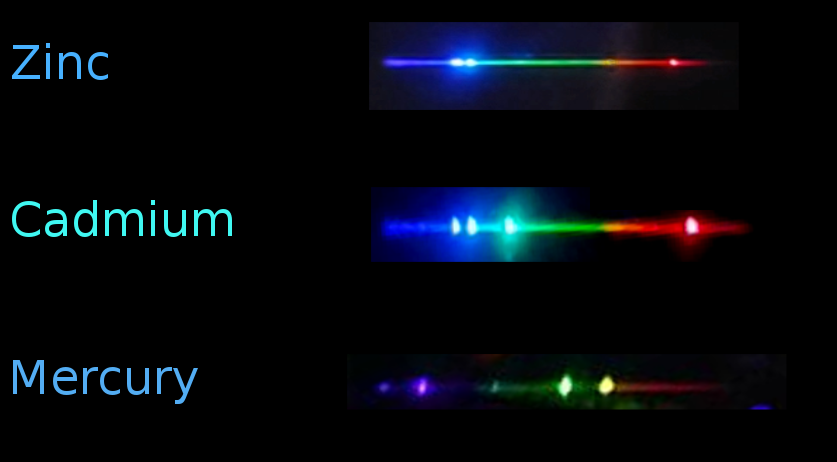
\includegraphics{images/line_spectra.png}
	\caption{Line spectra for various different elements. There are distinct wavelengths where there is a peak of emission. } 
	\labfig{line_spectra}
\end{marginfigure}

Attempting to match experimentally measured spectra, Bohr proposed that these orbits were quantized such that the angular momentum of the electron were integer multiples of $\hbar = h/(2\pi) $

\begin{equation}
	mvr = n\hbar \label{eq: quant}
	\end{equation}

where $n = 1,2,3,... $. Here, Bohr indeed finds that the same Planck constant that had been the key to understanding photons and blackbody radiation should be used here! The circular orbit requires that the centripetal force equal the electrostatic force between the electron of charge $ -e$ and nucleus (for Hydrogen) of charge $ e $:

\begin{marginfigure}[0cm]
	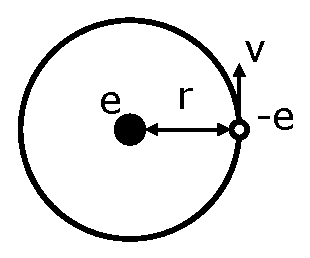
\includegraphics{images/chap1_atom_model.eps}
	\caption{A simplified model of the Hydrogen atom where an electron circularly orbits a proton at radius $ r $, and velocity $ v $.} 
	\labfig{atom_model}
\end{marginfigure}

\begin{equation}
	\frac{mv^2}{r} = \frac{e^2}{4\pi\epsilon_0 r^2} \label{eq:circ}
\end{equation}

Combining equations \ref{eq: quant} and \ref{eq:circ}, we can solve for the unknowns, $ v $ and $ r $ of the orbits:

\begin{equation}
v = \frac{e^2}{4\pi\epsilon_0 n\hbar}, r = \frac{n^2\hbar^2 (4\pi\epsilon_0)}{me^2}.
\end{equation}

The energy of the orbit is given by the kinetic plus the potential energy:

\begin{align}
	E &= \frac{mv^2}{2} - \frac{e^2}{4\pi\epsilon_0 r } \\
	&= -\frac{m e^4}{2(4\pi\epsilon_0)^2 n^2\hbar^2} = -\frac{\text{Ry}}{n^2}
\end{align}

where the Rydberg constant is defined from this formula. Remarkably, this simple model, along with this phenomenological quantization that depends on $ h $, does in fact agree with experiment and agrees with a more sophisticated model that we will develop later in this book. This quantization of energy, first seen in atoms is key to understanding many physical phenomena as well as designing technologies that are used everyday. 

\section{Everyday Quantum Mechanics}

The idea that energy levels in atoms and molecules are discretized is leveraged in many modern technologies. Discretization leads to atoms and molecules having particular absoprtion and emission transition frequencies. In contrast to incandescent light bulbs, which produce a continuous (white) light spectrum from heat\sidenote{A hot light bulb can be approximated as a blackbody}, neon lights use neon gas to give off a distinctive orange glow. Other so called ``neon lights" use hydrogen for purple-red light or mercury for blue light. In all these cases, the gas is ionized via \textit{electricity}, and then they relax to lower energy states emitting particular wavelengths. A more controlled emitter and the basis for many modern lasers are based on semiconductors. Even in the solid state, quantum mechanics predicts a "band-gap", or a gap in the energy spectrum, preferentially allowing for emission at a particular frequency. LED (light-emitting diode) lights use a combination of laser diodes at different frequencies to produce white (or apparently white) light of different "temperatures". The reason LED lights are far more efficient than incandescent ones is precisely the ability to concentrate the energy into particular frequencies combined with the human eye's lack of need for a continuous spectrum. We see white just fine, even if it's actually only a few wavelengths put together\sidenote[][-6mm]{In many cases, it's only 3! The so-called RGB color encoding comes from this idea.}. 

Concentration of energy at a particular frequency is a simplified definition for a laser\sidenote[][]{A laser is an acronym for \textbf{l}ight \textbf{a}mplification by \textbf{s}timulated \textbf{e}mission of \textbf{r}adiation. The stimulated here, in some sense, refers to a transition frequency being favored. Lasers are said to emit \textit{coherent} light, compared to a light bulb's \textit{incoherent} light. Higher quality lasers often have a smaller \textit{linewidth}, which describes exactly how narrow their spectrum is. Typical semiconductor lasers for research use have linewidths of 1 MHz or lower. Laser pointers can have linewidths of a few nanometers. Visible light has frequencies of 100s of THz (or wavelengths of 100s of nanometers), so it is quite remarkable how concentrated coherent light from a laser is! It is worth noting that another requirement typical for a laser is a good spatial \textit{mode}. In other words, lasers should propagate in a straight line, and not diverge too much. LEDs for lighting do not have this requirement, since it would be hard to light up a room with individual laser beams.}. Lasers have seen use as barcode scanners where the reflection is measured to determine the pattern of black and white that form a barcode. The same principle is also used in security systems where a blocked laser beam indicates an obstruction, which could signal a thief in your home. When you make a phone call with your cellphone, a \textit{proximity sensor} uses a infrared laser to sense that you are close to your phone and therefore locks your screen to prevent "ear touches". This concentration of energy in a laser can also be used to heat up objects. Have you ever tried to kill an ant with a magnifying glass in the sun? In this case, you are concentrating the energy from the sun. High power lasers are used in laser cutting, which can even cut through steel. 

High powers are required when an object does not absorb very much in the frequency range of your source. However, as we have discussed atoms and molecules have very particular frequencies. Water is known to have transitions in the microwave region, which is how the modern microwave works. It targets the frequency of a transition in water around 2.45 GHz, causing the water molecules to heat up and warm up your food. It is dangerous to microwave metal, precisely since it does not have a transition and this frequency and will reflect the powerful waves that your microwave emits, causing other areas of the microwave to be hit by the radiation.

The selectivity of radiation also allows for non-invasive imaging that is essential in modern medicine. Our skin reflects visible light\sidenote{Though not the same can be said about our friend \textit{C. elegans}.}, but it allows radio frequencies through just fine. This transparency to radio frequencies allows this radiation to probe structures \textit{inside} our bodies. It turns out the nuclei of hydrogen (protons) have transitions in these radio frequencies. Since hydrogen is prevalent in the body in many compounds, radio frequencies can be used to measure water and fat content in the body\sidenote[][-30mm]{If you've ever taken a MRI, you may have realized that you need to be placed into a big magnet. This giant magnet is required to create the discrete spectrum needed for spectral selectivity. It is worth noting that the chemical environment of the protons (what molecule the protons are a part of) also impacts these very precise frequencies. Chemists use this fact all the time in a technique called nuclear magnetic resonance (NMR) to fingerprint their compounds.}. This imaging technique is known as magnetic resonance imaging (MRI) and is a key diagnostic tool for soft-tissue, which does not have the type of crystalline solid structure to diffract x-rays. MRI imaging has been used in joints to identify tears in ligaments, but also in the brain to identify the onset of Alzheimer's disease. 


\begin{marginfigure}[0cm]
	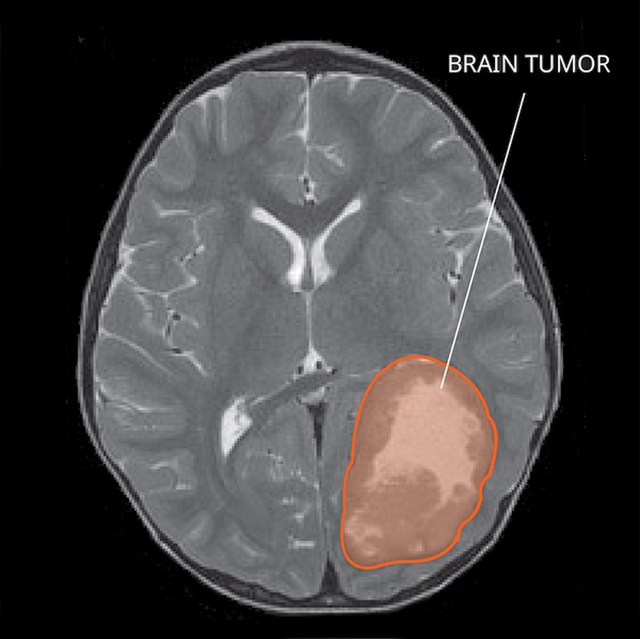
\includegraphics{images/brain_mri.jpg}
	\caption{A MRI of the brain showing a brain tumor.} 
	\labfig{brain_mri}
\end{marginfigure}


These particular examples just scratch the surface of how quantum phenomenon \textit{are} present in our everyday lives. As we progress in this book, other relevant examples will be brought up when necessary. Since quantum mechanics is a very non-intuitive subject, I believe that real world examples are especially important to grasp the concepts. Plus, they are just really cool. 

\section{Summary}

Through many beautiful experiments starting from the 19th century and continuing to the modern day, quantum mechanics has been verified time and time again. Grossly non-intuitive, quantum mechanics posits that light, classically thought of as waves, requires a particle like description and likewise, electrons, classically thought of as particles, requires a wave like description. To understand the line spectra of atoms, a heuristic quantization condition was introduced by Bohr. Although we did not elaborate here, quantization can be seen as a consequence of the wave-like behavior of particles analogous to how a string can only support a discrete set of frequencies, corresponding to the supported standing waves\sidenote{We will elaborate on this in the next chapter!}. Discretization of frequencies enables technologies like efficient lighting, lasers and medical imaging. Equating all of quantum mechanics to a discretization of energy is a gross oversimplification, but it is worth noting all the consequences that such a discretization of energy results in. With this prelude, I hope I have made you excited about the journey we are about to embark on. To really appreciate, understand and make use of quantum mechanics, we will need to engage in mathematical framework that will require concepts from linear algebra to calculus. However, I hope you always keep this introductory chapter in mind, and not get lost in the throws of mathematical calculation. The mathematics is describing a \textit{beautiful} set of experimental results and useful technologies. Enough prelude, let's go.
